\documentclass[11pt]{article}
\usepackage[utf8]{inputenc}
\usepackage{float}
\usepackage{bbm}
\usepackage{amssymb}
\usepackage{amsmath}
\usepackage{amsthm}
\usepackage{mathtools}
\usepackage{mathrsfs, enumerate}
\usepackage{appendix}
\usepackage[round]{natbib}
\usepackage[margin=1.5in]{geometry}
\linespread{1.25}
\usepackage{todonotes}
\usepackage{hyperref}
\graphicspath{{./figs/}}


\newtheorem{thm}{Theorem}[section]
\newtheorem{prop}{Proposition}[section]
\newtheorem{cor}{Corollary}[section]
\newtheorem{remark}{Remark}[section]
\newtheorem{lemma}[equation]{Lemma}
\newtheorem{assume}[thm]{Assumption}

\DeclareMathAlphabet\EuRoman{U}{eur}{m}{n}
\SetMathAlphabet\EuRoman{bold}{U}{eur}{b}{n}
\newcommand{\eurom}{\EuRoman}

\newcommand{\cB}{\mathcal{B}}
\newcommand{\cC}{\mathcal{C}}
\newcommand{\cF}{\mathcal{F}}
\newcommand{\cG}{\mathcal{G}}
\newcommand{\cH}{\mathcal{H}}
\newcommand{\cN}{\mathcal{N}}
\newcommand{\cP}{\mathcal{P}}
\newcommand{\cR}{\mathcal{R}}
\newcommand{\cS}{\mathcal{S}}
\newcommand{\cA}{\mathcal{A}}
\newcommand{\cX}{\mathcal{X}}
\newcommand{\cK}{\mathcal{K}}
\newcommand{\cT}{\mathcal{T}}
\newcommand{\cl}{\mathcal}
\newcommand{\cL}{\mathcal{L}}

\newcommand\indpt{\protect\mathpalette{\protect\indpT}{\perp}}
\def\indpT#1#2{\mathrel{\rlap{$#1#2$}\mkern2mu{#1#2}}}

\newcommand{\RR}{\mathbb{R}}
\newcommand{\EE}{\mathbb{E}}
\newcommand{\ZZ}{\mathbb{Z}}
\newcommand{\NN}{\mathbb{N}}
\newcommand{\PP}{\mathbb{P}}
\newcommand{\one}{\mathbf{1}}
\newcommand{\ep}{\varepsilon}

\newcommand{\bS}{\mathbb{S}}

\newcommand{\hc}{\hat{c}}
\newcommand{\hk}{{\hat{k}}}
\newcommand{\hf}{{\hat{f}}}
\newcommand{\hR}{\widehat{R}}

\newcommand{\tw}{\widetilde{w}}
\newcommand{\tk}{\tilde{k}}
\newcommand{\tX}{\tilde{\mat X}}
\newcommand{\tY}{\widetilde{Y}}
\newcommand{\tE}{\widetilde{E}}
\newcommand{\tOmega}{\widetilde{\Omega}}

\newcommand{\FDR}{\textnormal{FDR}}
\newcommand{\hFDR}{\widehat{\FDR}}
\newcommand{\hFDP}{\widehat{\FDP}}
\newcommand{\FDP}{\textnormal{FDP}}
\newcommand{\DP}{\textnormal{DP}}
\newcommand{\kn}{{\textnormal{Kn}}}
\newcommand{\ckn}{{\textnormal{cKn}}}
\newcommand{\eskn}{{\textnormal{EsKn}}}
\newcommand{\BH}{{\textnormal{BH}}}
\newcommand{\BY}{{\textnormal{BY}}}
\newcommand{\Bonf}{{\textnormal{Bon}}}
\newcommand{\hyb}{{\textnormal{Hyb}}}
\newcommand{\Do}{{\textnormal{do}}}


\newcommand{\simiid}{\overset{\text{i.i.d.}}{\sim}}
\newcommand{\eqd}{\overset{d}{=}}
\newcommand{\eqv}{\;\Leftrightarrow\;}
\newcommand{\sgn}{{\textnormal{sgn}}}

\newcommand{\pth}[1]{\left( #1 \right)}
\newcommand{\br}[1]{\left[ #1 \right]}
\newcommand{\cur}[1]{\left \{  #1 \right \}}
\newcommand{\vct}[1]{\boldsymbol{#1}}
\newcommand{\mat}[1]{\boldsymbol{#1}}
\newcommand{\abs}[1]{\left| #1 \right|}
\newcommand{\norm}[1]{\left\| #1 \right\|}
\newcommand{\set}[1]{\left \{  #1 \right \}}
\newcommand{\mon}[1]{\left \langle #1 \right \rangle}
\newcommand{\floor}[1]{\left \lfloor #1 \right \rfloor}
\newcommand{\ceil}[1]{\left \lceil #1 \right \rceil}
\newcommand{\Rset}{\mathbb{R}}
\newcommand{\pt}[1]{\dot{#1}}
\newcommand{\Var}{\text{Var}}

\newcommand{\mim}{\wedge}
\newcommand{\mam}{\vee}
\newcommand{\setcomp}{\mathsf{c}}
\newcommand{\toProb}{\stackrel{p}{\to}}
\newcommand*{\tran}{{\mkern-1.5mu\mathsf{T}}}


\newcommand{\note}[1]{{\color{red} #1 }}

\title{Causal Discovery Under the Potential Outcome Framework}
\author{Yixiang Luo}
\date{\today}

\begin{document}

\maketitle

\begin{abstract}
   Causal discovery is an important and common problem to the science community. The classical causal discovery approaches under the Directed Acyclic Graph model have essential difficulties in computational feasibility and determining the causal direction. In this project, I propose a model of doing causal discovery under the potential outcome framework and several immature methods created based on existing approaches. 
\end{abstract}


\section{Introduction}

\citet{gelman2011causality} points out that there are two types of causal queries:
\begin{enumerate}
    \item \textit{Forward causal questions}: the "what if" question, or the inference on the "effects of causes", i.e. what would happen if we do certain interventions?
    \item \textit{Reverse causal questions:} the "why" question, or inference on the "causes of effects", i.e. why do certain phenomena happen?
\end{enumerate}
The potential outcome model we learned in most statistical or econometrical classes is mainly used for the forward causal questions. As for the reverse question, a typical workflow under the potential outcome model is made clear by \citet{gelman2013ask}. In particular, the "why" question naturally arises when we observe a strange behavior that cannot be explained by the current model. For example, consider we observe the higher employee have higher salaries in the labor market while standard economic
models suggest that wages should be related to productivity, rather than height. Such anomaly would motivate researchers to introduce new variables like health and childhood nutrition into the model according to their domain knowledge and convert the reverse causal question to a forward causal question about the effect of the newly introduced causal variables. However, if we have little domain knowledge to propose reasonable causal variables, can we still tackle the reverse question? In particular, modern data science makes it possible to collect numerous data for a large number of variables that might be causes. Can we identify the causes from the data with a certain guarantee?

% multiple treatments

Causal discovery under the directed acyclic graph (DAG) framework seems to provide a good toolset for this problem. Most causal discovery approaches can be classified into two categories: the constraint-based approaches and the score-based approaches. The constraint-based methods such as the PC algorithm and the Fast Causal Inference algorithm \citep{spirtes2000causation} learn the undirected graph structure by recursively applying conditional independence test onto possible triples of variable sets in the graph. The causal directions are then partially detected by first identifying the colliders $a \rightarrow b \leftarrow c$ via conditional independence test and then using the so-called orientation propagation to impute the other directions. The score-based method such as the Greedy Equivalence Search algorithm \citep{chickering2002optimal} starts with an empty graph and adds the best directed edge at each step which increases fit the most measured by some quasi-Bayesian score.

There are two major difficulties in applying these causal discovery methods. First, as the number of variables increases, learning a complicated causal DAG quickly becomes computationally infeasible and requires a huge amount of data. Second, the causal directions are only partially identifiable up to the so-called Markov equivalent class. To fix the first problem, \citet{wang2013discovering} and \citet{wang2014discovering} propose to learn only the local causal graph around a variable of interest; \citet{xie2008recursive} and \citet{xie2006decomposition} decompose learning a large DAG into problems of learning many small DAG. However, the causal directions are still only partially identifiable in their methods. For the second difficulty, the newly developed LiNGAM methods \citep{shimizu2006linear,shimizu2011directlingam} shed a light on it as it can identify the causal directions except under 5 settings by assuming the noises are far from Gaussian or the causal relationship is nonlinear.

We shouldn't blame the algorithms for the above problems since these difficulties are from the essence of the causal DAG model. Unlike the simple potential outcome model, the DAG model requires knowing a complicated graph to make an inference. Moreover, it is impossible to identify a causal direction if only the values of two variables are observed, which lies in the heart of the direction identifiability problem in DAG causal discovery. However, the potential outcome model naturally doesn't have this issue as it decides the causal direction by domain knowledge. Hence a natural idea is, can we do causal discovery under the potential outcome model and enjoy its advantages? In particular, for the cases where we have domain knowledge of the causal order of the variables, e.g. ordering them by the time when they are measured, but little idea of which variables are potential causes, is there a way to identify the promising causes and their effect based on the observational data? In this project, I'll explore some ideas for it.

The rest of this paper is arranged as follows.

\section{Formulation and assumptions}%
\label{sec:formulation_and_assumptions}

\subsection{A motivating example}%
\label{sub:a_motivating_example}

Let's start with an example that motivates the formulation of the problem. Consider we want to investigate why do some people make more money than others at the age of 50. And we have the following observational data.
\begin{enumerate}
    \item At birth: the SNPs (genes) of the person, the monthly family income at birth.
    \item At age of 12: the height, the graduation exam grades at primary school, the monthly family income when the final exams take place, how good is the environment of the city where the person lives.
    \item At age of 18: the university the person enters, the BMI.
    \item At age of 30: the hours the person sleeps, the number of friends the person has.
    \item The outcome of interest: the income at age of 50.
\end{enumerate}

The key feature of the above variables is that they are measured in a sequence of time. It leads to two consequences:
\begin{enumerate}
    \item the lower level variables (measured earlier) might be causes of the higher-level variables (measured later) but the reverse is automatically not true. In other words, the causal direction is clear between different levels of variables.
    \item the variables of the same level (measured at the same time) may be correlated (have common causes) but have no causal effect on each other.
\end{enumerate}
The second point is a bit subtle. Let me illustrate it with some examples. Consider the SNPs. It is known that some SNPs can have a strong correlation as the corresponding genes are next to each other in the DNA sequence. However, they have no causal effect on each other in the sense that if we edit one gene by, say, CRISPR, the other gene wouldn't change. Another example is the primary school graduate exam grade and the monthly family income when the exam takes place. They might have common causes, e.g. the unemployment of a parent a year ago might affect the study environment of the child thus the exam grades as well as the later family income. But the family income when the exam takes place is expected to have no or at least very little causal effect on the exam grades.

In general, the non-causality between the variables of the same level relies on that they are measured at the same time. This makes the formulation of the problem convenient but weakens the causal conclusion we can draw. For instance, suppose we find that "the monthly family income when the primary school graduation exam takes place" ("instant income" for short) is a cause and has a causal effect of 10 units. It is dangerous to claim that if we intervene and give a certain amount of money to that family in that month, the child would make 10 units more money at his/her age of 50. In fact, the instant income should be treated as a proxy of "the family economic status around that time" ("period income" for short). In the causal inference language, the period income is an unobserved common cause of the instant income and the outcome of interest. Importantly, the instant and period income are a "cause" of each other. Hence the real causal effect should be weaker than we estimate if the latent period variable covers a much longer time period than the instant variable. And in this sense, these instant variables automatically break the unconfoundedness assumption to a certain extent. However, if we insist on being honest to the reality and adopting the period variables, it's natural to see complicated mutual causal effects among many variables, which is beyond the ability of many state-of-the-art methods. I believe using instant variables is a reasonable and mathematically clean way to simplify the real situation.

\subsection{Notations and formulation}%

In this section, I'll formalize what we have seen in the example above.

Let $X^{(l,k)}$ be the possible causal variables we want to investigate, where $l = 1, 2, \ldots, L$ is the index of $L$ levels and $k = 1, 2, \ldots, K_l$ is the index of the $K_l$ variables within each level $l$. For instance, variable "the height" in the example above is the first variable of level 2. So it is denoted as $X^{(2,1)}$. For simplicity, let
\[ j(l,k) = \sum_{s=1}^{l-1} K_s + k \]
be the one dimensional index of the $(l,k)$-th variable so $ X^{(j)} := X^{(l,k)}$ and
\[ m = \sum_{s=1}^l K_s \]
be the total number of variables. Define $X = \pth{X^{(j)}}_{j = 1, \ldots, m}$ as the vector of all variables and
\[V^{(l,k)} = \pth{X^{(s,t)}: \; s \leq l, (s, t) \neq (l, k)}\]
as the vector of variables having no higher level than $X^{(l, k)}$ excluding $X^{(l, k)}$, ordered by $j$.

Denote the outcome of interest as $Y$. The causal effect is probably easier to think about in the language of the DAG model. But let's write down the potential outcome
\[ Y(\Do(X^{(l,k)}) = x) \]
as the outcome if we assign treatment $X^{(l,k)} \leftarrow x$ without interfering the pre-treatement variables. For simplicity of notation, let $Y^{(l,k)}(x) := Y(\Do(X^{(l,k)}) = x)$ be its succinct version. Formally, the potential outcome $Y^{(l,k)}(x)$ is nothing but an "arbitrary" random function of $x$ in the science table. The causal effect of $X^{(l,k)}$ is define as some functional on $Y^{(l,k)}(x)$. For example, if $X^{(l,k)}$ is binary and we employ the ATE, then the causal effect is
\[ \tau^{(l,k)} =  \EE \br{Y^{(l,k)}(1) - Y^{(l,k)}(0)}. \]
As before, I use $j$ as the one-dimensional alternative for the index $(l,k)$ and define $Y(x) = \pth{Y^{(j)}(x_j)}_{j = 1, \ldots, m}$ as the vector of potential outcomes, where $x = (x_1, x_2, \ldots, x_m) \in \cX$ is a vector of the assigned treatment and $\cX = \prod_{j=1}^m \cX^{(j)}$ is its range.

Suppose we observe
\[ (X_i, Y_i(\cX)) \simiid (X, Y(\cX)) \]
for unit $i = 1, 2, \ldots, n$, where $Y(\cX)$ denotes the joint vector over all values of $x \in \cX$. The observed outcome
\[ Y_i := Y_i^{(j)}(X_i^{(j)}), \quad \forall j. \]
For simplicity, I write the observed $X$-variables as a matrix $\mat X \in \RR^{n \times m}$ with $\mat X_{ij} := X_i^{(j)}$.

The goal is to estimate the treatment effect of each variable $X^{(l,k)}$ on $Y$ and select the causal variables with a certain guarantee. Here I pick the finite sample false discovery rate (FDR) \citep{benjamini1995controlling} control as the target. We can phrase the causes selection problem as hypothesis testing:
\[ H_j: \tau^{(j)} = 0. \]
Let $\cH_0$ be the set of true null hypothese and $\cR$ be the set of hypotheses we reject. Then the false discovery proportion (FDP) is defined as
\[ \FDP = \frac{|\cR \cap \cH_0|}{|\cR| \mam 1}. \]
And FDR is defined as $\FDP = \EE[\FDP]$. The goal is to control $\FDR \leq \alpha$ for some given $\alpha \in (0,1)$.

\subsection{Assumputions}%
\label{sub:assumputions}

Here I make my assumptions clear.

The first assumption is rephrasing the key feature we see in the motivating example. It is not a component in the potential outcome framework and is informal. I include it here as it makes the PO framework and the other assumptions more plausible.
\begin{assume}[causal ordering]
    $X^{(l,k)}$ happens no earlier than any $X^{(s,t)}$ for $s \leq l$. And $Y$ happens the last.
\end{assume}

The rest assumptions are basically standard in the potential outcome model.
\begin{assume}
    Stable Unit Treatment Value Assumption.
\end{assume}

\begin{assume}[uniform ignorability]
    \[ X^{(l,k)} \indpt Y^{(l,k)}(x) \mid V^{(l,k)}, \quad \forall x \in \cX^{(l,k)} \]
    holds for all $(l,k)$.
\end{assume}
The uniform ignorability assumption is not hard to understand. Suppose we want to investigate the causal effect of variable $X^{(l,k)}$ (view it as treatment). Then based on the causal ordering assumption, the pre-treatment variables are the elements in $V^{(l,k)}$ and thus can be viewed as covariates. Then the uniform ignorability assumption reduces to the usual ignorability assumption. In the language of the DAG framework, it means any common causes of $X^{(l,k)}$ and $Y$ are blocked by $V^{(l,k)}$.

\begin{remark}
    Is the uniform ignorability assumption plausible? Indeed, it is much stronger than the usual ignorability assumption that applies to a single treatment. But just as in the usual case, the assumption becomes more plausible if we include many more possible causes into $X$. And this is exactly the case we are facing here: we put numerous variables that might be causes of $Y$ into $X$ and try to figure out the true causes among them. And even if the assumption doesn't hold, we find good proxies for the actual causes which may guide further research.
\end{remark}

\section{Proposed methods}%
\label{sec:proposed_methods}

In this section, I'll explore some ideas to solve the problem. The first subsection proposes a naive method under the general setting. And the next subsection discusses some weakness of the general method and propose possible solutions under the Gaussian graphical model.

\subsection{General setting}%
\label{sub:general_setting}

In this subsection, I make no model assumption and try to tackle the problem under the general setting. I have little experience in handling treatments of multi-level or continuous value. Hence here when investigating the treatment effect of $X^{(l,k)}$, I dichotomize it and employ the ATE. Formally, this is to define the treatment effect as (suppressing the superscript $(l,k)$ on $X$, $V$, $Y$, $\tY$, $w$, and $\tau_d$ for simplicity)
\[ \tau_d := \EE \br{\tY(1) - \tY(0)}, \]
where
\[
    \tY(z) := \int w(x; z) Y(x), \quad
\]
\[ 
    w(x; z) := \one_{z=1, \, x \geq \bar x} \int d\,P_V(V) \, \frac{d \,P_{X|V}(x)}{P_{X|V}(x \geq \bar x)} + 
    \one_{z=0, \, x < \bar x} \int d\,P_V(V) \, \frac{d \,P_{X|V}(x)}{P_{X|V}(x < \bar x)},
\]
and $\bar x = \EE[X]$, $P_{X|V}$ is the conditional distribution of $X$ given $V$, and $P_V$ is the marginal distribution of $V$. In other words, the dichotomized potential outcome $\tY(x)$ is a weighted average of the original potential outcome $Y(x)$, where the weight is determined based on the proportion of $x$ among all $x$ that falls into the same category.

\subsubsection{inference on individual treatment}%
\label{subsub:causal_inference_for_individual_treatment}

Consider inferring the treatment effect of a single variable $X^{(l,k)}$. Again, I suppress the superscript $(l,k)$ for simplicity when there is no ambiguity.

As discussed before, the uniform ignorability assumption reduces to the usual ignorability assumption when we view $X$ as treatment and $V$ as covariates. And it's not hard to see the dichotomized potential outcomes still satisfy the ignorability assumption
\[
    Z \indpt \tY(z) \mid V, \quad z = 0,1, \quad
    \text{ where } Z := \one \set{X > \bar x}
\]
Hence we can adopt the usual causal inference methods in the potential outcome framework. As a final project, I employ three main approaches for the observational study we learned in the class.

\begin{enumerate}
    \item \textit{IPW/Hajek estimator}.
        \[
            \hat{\tau}_d^{\text {hajek}}=\frac{\sum_{i=1}^{n} \frac{Z_{i} Y_{i}}{\hat{e}\left(X_{i}\right)}}{\sum_{i=1}^{n} \frac{Z_{i}}{\hat{e}\left(X_{i}\right)}}-\frac{\sum_{i=1}^{n} \frac{\left(1-Z_{i}\right) Y_{i}}{1-\hat{e}\left(X_{i}\right)}}{\sum_{i=1}^{n} \frac{1-Z_{i}}{1-\hat{e}\left(X_{i}\right)}},
        \]
        where $\hat e$ is the estimated propensity score.

        An estimator of the variance $\hat V^{\text{hajek}}$ is obtained by bootstrap.
    \item \textit{Doubly robust estimator} with linear model.
        \[ \hat{\tau}^{\mathrm{dr}}=\hat{\mu}_{1}^{\mathrm{dr}}-\hat{\mu}_{0}^{\mathrm{dr}}, \]
        where
        \[
            \hat{\mu}_{1}^{\mathrm{dr}}=\frac{1}{n} \sum_{i=1}^{n}\left[\frac{Z_{i}\left\{Y_{i}-\hat \mu_{1}\left(X_{i}\right)\right\}}{\hat e\left(X_{i}\right)}+\hat \mu_{1}\left(X_{i}\right)\right],
        \]
        \[
            \hat{\mu}_{0}^{\mathrm{dr}}=\frac{1}{n} \sum_{i=1}^{n}\left[\frac{\left(1-Z_{i}\right)\left\{Y_{i}-\hat \mu_{0}\left(X_{i}\right)\right\}}{1- \hat e\left(X_{i}\right)} + \hat \mu_{0}\left(X_{i}\right)\right]
        \]
        and $\hat \mu_1$ is the predicted value of $Y$ by linear regression on the treated group and $\hat \mu_0$ is similar but on the control group.

        Again, an estimator of the variance $\hat V^{\text{dr}}$ is obtained by bootstrap.
    \item \textit{Matching based on propensity score}.
       
        I adopt the 1-nearest matching measured by the estimated propensity score. The biased corrected estimator $\hat \tau^{\text{mbc}}$ for the treatment effect and $\hat V^{mbc}$ is employed. The long formulas are omitted here for simplicity. Please see lecture notes section 15 for them.
\end{enumerate}

\begin{remark}
    As we infer the treatment effect for a hight-level variable $X^{(l,k)}$ with large $l$, the pre-treatment covariates $V^{(l,k)}$ may contain too many variables so that conditioning on $V^{(l,k)}$ may cause the non-overlap issue. A natural idea to solve this is to do the individual inference sequentially from low level to high, and don't condition on those showing no causal effect to the outcome. But this is invalid since
    \begin{enumerate}
        \item Due to the nature of hypothesis testing, we can only claim there exists a causal effect with certain confidence but cannot claim the null hypothesis, there is no causal effect, is true even if we don't reject the null.
        \item What we estimate is the total treatment effect rather than the direct treatment effect. Hence it is possible that $X^{(1,1)}$ has negative direct effect on $Y$ and positive effect via $X^{(1,1)} \to X^{(2,2)} \to Y$ and show zero total effect. But when doing inference on $X^{(2,2)}$, we definitely should condition on $X^{(1,1)}$.
    \end{enumerate}
    Fortunately, this problem would be relieved largely if we always use the propensity score as the covariate to condition on. By doing so, the non-overlapping issue happens only if the covariates are too predictive to the treatment variable. If we believe the causal DAG is sparse, then including many nuisance variables doesn't really make the covariates more predictive of the treatment.
\end{remark}

\subsubsection{multiple testing procedures}%
\label{subsub:multiple_testing_procedures}

Once we have an estimator $\hat \tau^{(j)}$ for the treatment effect of $X^{(j)}$ and an estimator $\hat V^{(j)}$ for the variance of $\hat \tau^{(j)}$, we can obtain an asymptotically valid p-value
\[ p_j = 2 \cdot \Phi \pth{-\abs{\frac{\hat \tau^{(j)}}{\sqrt{\hat V^{(j)}}}}}, \]
by the central limit theorem (if holds), where $\Phi$ is the CDF of the standard normal distribution.

Then the causal selection problem becomes the classical multiple testing problem with FDR control. \citet{benjamini1995controlling} proposed the commonly used $\BH(\alpha)$ procedure for this purpose, which rejects
\[ \cR = \set{j: p_j \leq \frac{\alpha R}{m}}, \]
where
\[ R = \max \set{r: \frac{m p_{(r)}}{r} \leq \alpha} \]
and $p_{(r)}$ is the $r$-th smallest among all the p-values
\[ p_{(1)} \leq p_{(2)} \leq \cdots \leq p_{(m)}. \]

The $\BH(\alpha)$ procedure gives provably FDR control if the p-values are independent or satisfy certain positive dependence called PRDS \citep{benjamini2001control}. However, due to the dichotomization and the unknown causal relationship between the $X$ variables, the p-values we get have a complicated and unknown dependency. Hence we need to adopt the more conservative method $\BY(\alpha) = \BH(\alpha / L_m)$ proposed by \citet{benjamini2001control}, where
\[ L_m = \sum_{k=1}^m \frac 1k \approx \log m, \]
if we want to control FDR with a theoretical guarantee.

The last concern is that we only have (maybe) asymptotically valid p-values. The following proposition should help.

\begin{prop} \label{prop:asymp}
    Suppose $\PP(p_j \leq t) \leq t + \ep$ for all $j$ and some $\ep \geq 0$. Then the $\BY(\alpha)$ procedure based on these p-values control FDR at $\alpha + m L_m \ep$.
\end{prop}
\begin{proof}
    Let $\cR$ denotes the rejection set of $\BH(\alpha)$ and $R = |\cR|$ for simplicity of notation. Define
    \[
        S_i=\left\{\begin{array}{cl}
1, & p_{i} \leq \frac{\alpha}{m} \\
\frac{1}{2}, & \frac{\alpha}{m}<p_{i} \leq \frac{2 \alpha}{m} \\
\vdots & \\
\frac{1}{m}, & \frac{\alpha(m-1)}{m}<p_{i} \leq \alpha \\
0, & p_{i}>\alpha
\end{array}\right..
    \]
    Since $\PP(p_j \leq t) \leq t + \ep$, we have
    \[ 
        \mathbb{E}\left[S_{i}\right] \leq\left(1+\frac{1}{2}+\ldots+\frac{1}{m}\right) \cdot \pth{\frac{\alpha}{m} + \ep} = L_m \cdot \pth{\frac{\alpha}{m} + \ep}.
    \]
    Then we have
    \begin{align*}
        \FDR = \sum_{i \in \cH_{0}} \mathbb{E} \left[\frac{\one \left\{p_{i} \leq \frac{\alpha R}{m}\right\}}{R \mam 1}\right]
        \leq \sum_{i \in \cH_{0}} \mathbb{E} \br{S_i}
        \leq L_m (\alpha + m \ep),
    \end{align*}
    where the first inequality is by 
    \[
        p_{i} \leq \frac{\alpha R}{m} \quad\Rightarrow\quad S_{i} \geq \frac{1}{R} \quad\Rightarrow\quad \frac{\one \left\{p_{i} \leq \frac{\alpha R}{m}\right\}}{R} \leq S_{i}.
    \]
    Finally, noticing $\BY(\alpha) = \BH(\alpha / L_m)$, the propostion is proved.
\end{proof}

It's not hard to see that if the CLT holds and $\hat V^{(j)}$ is conservative, then the condition in Proposition \ref{prop:asymp} holds with a large enough $n$.


\subsection{Gaussian graphical model}%
\label{sub:gaussian_graphical_model}

In this section, I consider a widely adopted model assumption and try a different idea to tackle the problem.

\subsection{Formulation}%
\label{sub:formulation}

Assume $(X, Y)$ obeys the Gaussian graphical model, i.e they jointly follow a multivariate Gaussian distribution. This allows us to write $Y$ as a Gaussian linear model of any subset of $X$: for any $\cL \subseteq [m]$, we can write
\begin{equation}\label{eq:linear}
    Y = \sum_{j \in \cL} X^{(j)} \beta_j^\cL + a^\cL + \ep^\cL
\end{equation}
where $a^\cL$ is a constant intercept and $\ep^\cL$ is a Gaussian noise independent of $X$. The superscript $\cL$ indicates these variables may vary as $\cL$ varies.

Now come back to the causal inference. Under the potential outcome model with ignorability assumption, formally, the most general definition of existing a causal effect is that conditioning on the pre-treatment variables, the treatment is not independent with the outcome
\[ X^{(l,k)} \not \indpt Y \mid V^{(l,k)}. \]
With the linear model \eqref{eq:linear}, it's equivalent to have $\beta^{\cL(j)}_j \neq 0$ in
\begin{equation} \label{eq:model}
    Y = \sum_{i \in \cL(j)} X^{(i)} \beta_i^{\cL(j)} + a^{\cL(j)} + \ep^{\cL(j)},
\end{equation}
where
\[ \cL(j) = \set{i: \; i \leq \min \set{\sum_{s=1}^l K_s: \; \sum_{s=1}^l K_s \geq j}} \]
is the set of the one-dimensional variable indeces that has level no higher than $X^{(j)}$. In words, we only need to include $X^{(l,k)}$ and $V^{(l,k)}$ in the linear model when infering the total treatment effect of $X^{(l,k)}$. And this correspond to the regression based method for linear model in the classical causal inference.

Formally, we can rephrase our causal discovery problem as again a multiple hypotheses testing on
\[ H_j: \; \beta^{\cL(j)}_j = 0, \quad j \in [m], \]
where the $m$ different $\beta^{\cL(j)}_j$ come from $L$ different linear models of the form \eqref{eq:model}.

\subsection{Modify the knockoff method}%
\label{sub:the_knockoff_method}

The knockoff method \citep{barber15, candes2018panning} is shown to have higher power than the BH method under many practical settings in selecting the nonzero $\beta$ coefficients in a Gaussian linear model with FDR control. I'll use the fixed-X version of the method which suits our goal the best.

Consider we observe $Y \in \RR^n$ and $\mat X \in \RR^{n \times m}$ in the model
\[ Y = \mat X \beta + \ep. \]
To select the $\beta_j \neq 0$, the knockoff method constructs a so-called knockoff matrix $\tX$ matrix satisfying
\[
\br{\mat X \; \tX}^T \br{\mat X \; \tX}
=\left[\begin{array}{cc}
\mathbf{X}^{\top} \mathbf{X} & \mathbf{X}^{\top} \tilde{\mathbf{X}} \\
\tilde{\mathbf{X}}^{\top} \mathbf{X} & \tilde{\mathbf{X}}^{\top} \tilde{\mathbf{X}}
\end{array}\right]=\left[\begin{array}{cc}
\boldsymbol{\Sigma} & \boldsymbol{\Sigma}-\operatorname{diag}\{\mathbf{s}\} \\
\boldsymbol{\Sigma}-\operatorname{diag}\{\mathbf{s}\} & \boldsymbol{\Sigma}
\end{array}\right] := \mathbf{G}
\]
for some vector $\vct s \geq 0$ that makes $\mat G$ semi-positive definite. The idea is that the knockoff feature $\tX_j$ mimics the true feature $\mat X_j$ in its correlation structure with the other features but not the outcome. Hence if $\beta_j = 0$, a feature selection method like lasso should not be able to distinguish $\mat X_j$ with its knockoff $\tX_j$, which serves as a negative control for FDR.

In particular, knockoff then run Lasso with different penalty level $\lambda$ in the augmented regression problem $Y \sim [\mat X \; \tX]$ and define
\begin{gather*}
    W_j = (\text { largest } \lambda \text { such that } \mathbf{X}_{j} \text { or } \tilde{\mathbf{X}}_{j} \text { enters Lasso path }) \\
    \times\left\{\begin{array}{ll}
+1 & \text { if } \mathbf{X}_{j} \text { enters before } \tilde{\mathbf{X}}_{j} \\
-1 & \text { if } \mathbf{X}_{j} \text { enters after } \tilde{\mathbf{X}}_{j}
\end{array}\right..
\end{gather*}
Then knockoff reject
\[\cR = \left\{j: W_{j} \geq T\right\},\]
where
\[ T = \min \left\{t>0: \frac{1+\#\left\{j: W_{j} \leq-t\right\}}{\#\left\{j: W_{j} \geq t\right\}} \leq \alpha \right\}. \]

Our causal selection problem is different from the original feature selection goal of knockoff in the following two aspects.
\begin{enumerate}
    \item Our coefficient $\beta^{\cL(j)}_j$ are from $L$ different model rather than a single linear model.
    \item In one particular model \eqref{eq:model}, only the features/variables having the same level with $X^{(j)}$ should be considered to be selected.
\end{enumerate}

Here I propose a modified knockoff method to tackle our causal selection problem. For each level $l = 1, 2, \ldots, L$, let $\cL_l$ be the indeces set of all variables having level no higher than $l$, e.g. $\cL_l = \cL(j)$ if $X^{(j)}$ has level $l$. Let the initial selection set $\cR = \emptyset$. Iterate
\begin{enumerate}
    \item Let $Y = (Y_i)_{i \in [n]}$ be the vector of the observed outcome among $n$ units. Let $mat X^{\cL_l}$ be the matrix of the observed variables having level no higher than $l$.
    \item Run knockoff at FDR level $\alpha / L$ with a properly chosen $\vct s$ such that $\vct s_j = 0$ for all $j$ such that $X^{(j)}$ has level less than $l$. By doing so, we will automatically have $W_j = 0$ and hence only the features/variables having the same level as $l$ are considered to be selected. Denote the selection set as $\cR_l$.
    \item update $\cR \leftarrow \cR \cup \cR_l$.
\end{enumerate}

And we can show it has provable FDR control.
\begin{thm}
    The modified knockoff method controls FDR.
\end{thm}
\begin{proof}
    \begin{align*}
        \FDR(\cR)
        &= \EE \br{\frac{|\cR \cap \cH_0|}{|\cR| \mam 1}}
        = \sum_{l=1}^L \EE \br{\frac{|\cR_l \cap \cH_0|}{|\cR| \mam 1}} \\
        &\leq \sum_{l=1}^L \EE \br{\frac{|\cR_l \cap \cH_0|}{|\cR_l| \mam 1}}
        = \sum_{l=1}^L \FDR(\cR_l)
        \leq \sum_{l=1}^L \frac{\alpha}{L}
        = \alpha
    \end{align*}  
\end{proof}

\begin{remark}
    Knockoff is known to perform well if the true model is sparse and the nominal FDR level is not too small. Otherwise, it might be worse than BH/BY. Hence I expect the modified knockoff method to perform well if we don't have too many levels of variables but have many variables in each level.
\end{remark}

\section{Simulation studies}%
\label{sec:simulation_studies}

In this section, I examine the proposed methods by numerical simulations. Due to the computational price, e.g. the doubly robust estimator requires $2m$ times model fitting for a single problem, and the time limit of this project, I'm only able to do the experiments on limited settings. But they should reveal typical behaviors of the methods.

Recall we have $m$ variables $X^{(j)}$ for $j = 1, 2, \ldots, m$ with each has its level. I generate the data via the causal DAG model with Gaussian linear model as follows.
\begin{enumerate}
    \item Create a Erdos-Renyi graph of $m+1$ nodes with the probability of assigning an edge to be $\pi_1 \in [0, 1]$. Treat the first $m$ nodes as $X$ and the last node as $Y$.
    \item Generate the level of each $X$ variable to make each level has about the same number of variables. For example, if we have $m=7$ and $L=3$, I assign $X^{(1)}, X^{(2)}, \ldots, X^{(m)}$ to have level
        \[1, 1, 2, 2, 3, 3, 3.\]
        Let $Y$ have the highest level $L+1$.
    \item If there is an edge between two nodes of different levels, then make it an directed causal edge from the lower level to the higher level.
    \item Let $pa(v)$ be the set of nodes that eject an edge into $v$, where $v$ can be either a $Y$ or a $X$ variable. Then from low level to high level, the value of $v$ is determined as
        \[ \text{value}(v) \leftarrow \sum_{w \in pa(v)} \mu(w,v) \cdot \text{value}(w) + N(0,1), \]
        where $\mu$ is the signal strength and $N(0,1)$ is an independent noise.
\end{enumerate}
In short, I adopt the Gaussian graphical model with sparsity level $\pi_1$. And the levels of $X$ variables are distributed evenly.

The existence of a causal effect is defined as rejecting
\[ H_j: \; X^{(j)} \not \indpt Y \mid V^{(j)}. \]
I'll compare the estimated FDR and power, defined as
\[
    \text{Power} := \EE[\frac{|\cR \cap \cH_1}{|\cH_1|}],\quad
    \cH_1 := [m] \setminus \cH_0,
\]
of the proposed methods.

In the experiments below, I set $m = 100$, $n = 400$ and $\pi_1 = 0.2$. $\mu$ is set to have value varies from $0.05$ to $0.3$. The "Wide", "Moderate", and "Long" structures correspond to set $L = 1, 4, 10$. The code to reproduce the results is available at \url{https://github.com/yixiangLuo/CDPO}. 

Figure \ref{fig:pos_signal} shows the estimated FDR and power of the proposed methods as signal strength increases. All methods control FDR empirically (The doubly robust estimator under the "Wide" structure exceeds a little bit But that can be explained by Monte-Carlo error).

\begin{figure}[!htb]
    \centering
    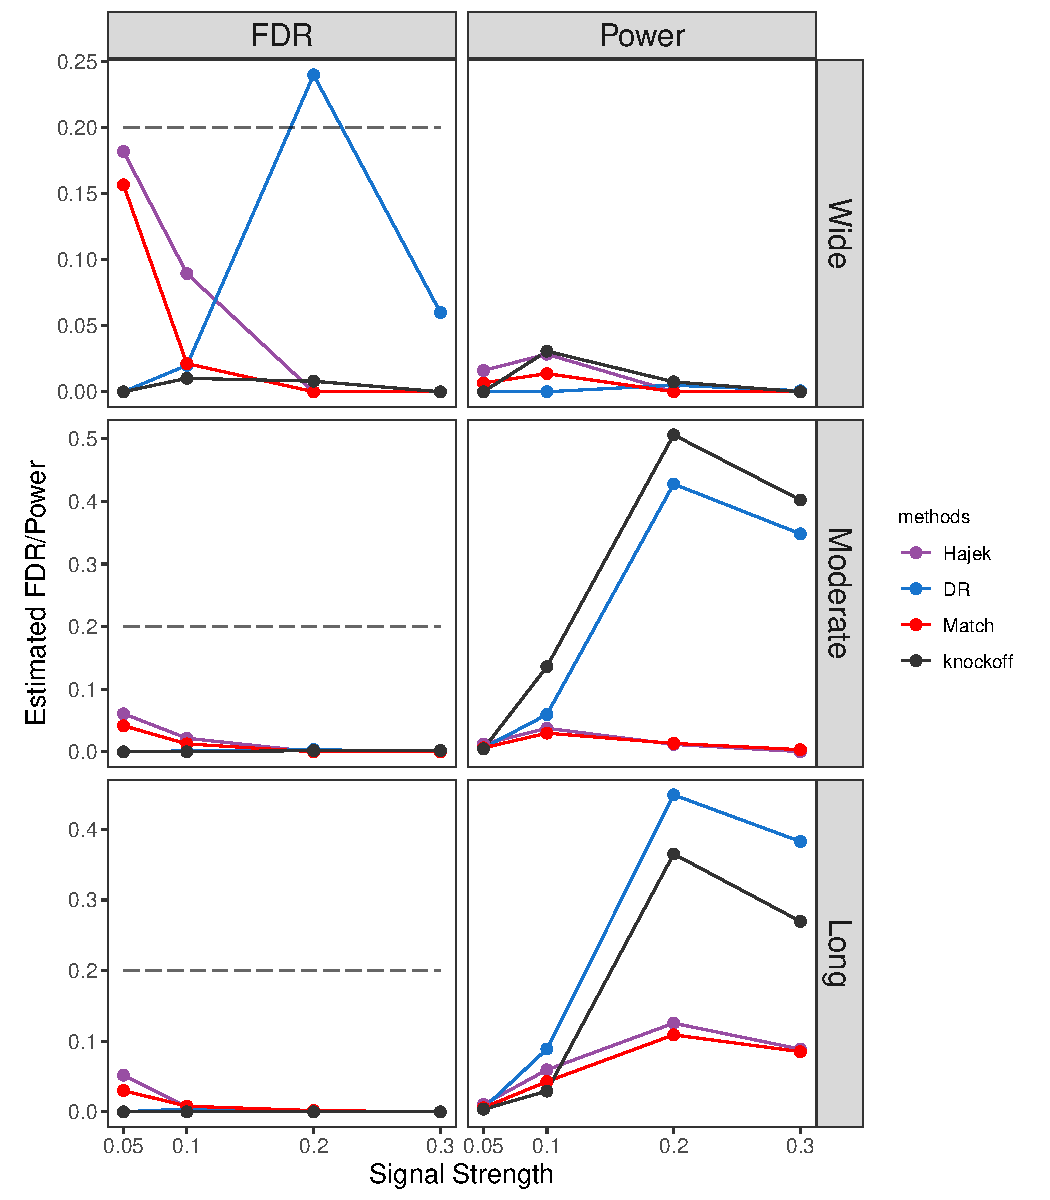
\includegraphics[width = 1\textwidth]{simu-pos_signal.pdf}
    \caption{Estimated FDR and power of the proposed methods as signal strength increases. $\alpha = 0.2$. All methods controls FDR empirically. The doubly robust estimator and the modified knockoff are among the best.}
    \label{fig:pos_signal}
\end{figure}

Some major takeaways from the figure:
\begin{enumerate}
    \item The doubly robust estimator and the modified knockoff are among the best. In particular, the modified knockoff method is better when the level structure is "wider" (more $X$ variables in the same level and less total number of levels), which is as expected. The powerless of all methods under the extremely wide setting (the "Wide" in the figure, which has $L=1$) remains a mystery and needs further investigation.
    \item As the signal strength increases after a certain point, e.g. $0.2$, the power decreases.
        For the ATE-based methods (Hajek, DR, and Match), this is because as the signal strength increases, the covariates $V^{(j)}$ become more predictive to the treatment variable $X^{(j)}$. Hence more estimated propensity scores tend to the extreme value $0$ or $1$ and hence the data point is swiped out. When the number of overlapped data points (propensity score $\in [0.1, 0.9])$ is less than say $10$, I enforce not to reject such $X^{(j)}$.
        For the modified knockoff method, I think it is because that the stronger positively correlated design matrix $\mat X$ introduces a larger whitening noise to knockoff, which is known as an important difficulty of the knockoff method.
\end{enumerate}

\section{Discussion}

In this project, I propose a new model of layered causal discovery under the potential outcome framework. The model is suitable when we have domain knowledge of the time ordering the variables but little clue of the causes of an outcome of interest.

Several approaches moderately modified from existing methods are proposed to tackle the problem. Numerical simulations show they work okay but not really well. Especially in the sense that as the signal strength increases, none of the methods would attain power $1$. This calls for further research on new methods that are really designed for this problem if the whole causal discovery story and framework make sense.




\bibliographystyle{plainnat}
\bibliography{biblio.bib}






% \appendix
% \section{Proofs}
% \label{app:proof}



\end{document}

